\documentclass[12pt]{article}

\usepackage[english]{babel}
% Set page size and margins
\usepackage[letterpaper,top=0.5cm,bottom=0.5cm,left=1cm,right=1cm,marginparwidth=0.5cm]{geometry}
\usepackage{listings, amsmath, caption,graphicx, xcolor, algorithm, algpseudocode}
\usepackage[colorlinks=true, allcolors=blue]{hyperref}
\lstdefinestyle{mystyle}{
    language=Python,
    basicstyle=\ttfamily\small,
    keywordstyle=\color{blue},
    commentstyle=\color{green!40!black},
    stringstyle=\color{purple},
    numbers=left,
    numberstyle=\tiny\color{gray},
    stepnumber=1,
    numbersep=5pt,
    backgroundcolor=\color{gray!5},
    frame=single,
    breaklines=true,
    breakatwhitespace=true,
    tabsize=4
}

\lstset{style=mystyle}

% \title{Assignment 4 Report}
% \author{Renwei Deng T12902101}

\begin{document}
% \maketitle

\section{Experiment settings}

\subsection{Hardware Specification \& Package version}
\begin{itemize}
    \item computation hardware: (cpu) intel i5
    \item \begin{center}
      \begin{tabular}{l|r}
            Package & Version \\\hline
            torch & 2.0.1 \\
            torchvison & 0.15.2 \\
            matplotlib & 3.8.0 \\
            python & 3.10.2
      \end{tabular}
    \end{center}
\end{itemize}

\subsection{How to use Grad-CAM for visualizing this model}
\begin{figure}[h]
    \centering
    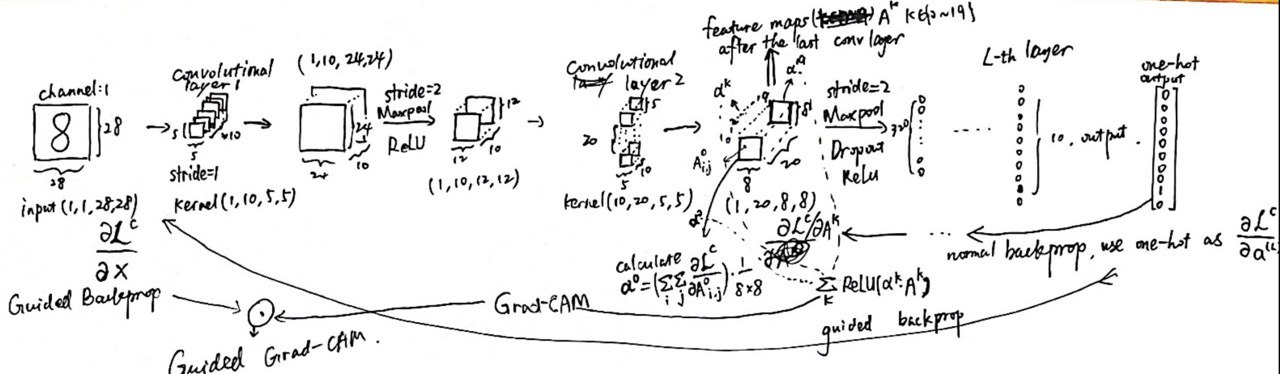
\includegraphics[width=1\linewidth]{../how.jpg}
    % \caption{\label{fig:how}}
    \end{figure}
\begin{enumerate}
    \item Grad-CAM: Expose feature maps in forward function in the given class. Then input each testing image to model to perform forward pass. After that, produce a one-hot vector as the partial derivatives of output to do the backprop. Finally, you can get gradients and activations from feature maps, with which you can perform operations to get Grad-CAM.
    \item GuidedBackprop: After gaining all the Grad-CAMs of testing images, it's time to register backward hook on all the layers of the model, in which you can manually specify how backprop should perform. In this context, we need to apply ReLU for each input gradient. Then after setting testing image to require gradients, input it to model and do the backprop. This time the backprop would automatically be guided. Lastly, collect the gradient from the image tensor.
    \item Guided Grad-CAM: For each testing image,after collecting its grad-CAM and guided gradient, simply element-wise multiply them.
\end{enumerate}

\subsection{Visually show the Grad-CAM of the given testing images}

Since I have 8 testing images, and each of them would be plotted 4 times(Raw, Grad-MAP, Guided Backprop, Guided Grad-MAP), so instead of profile, I choose a landscape layout for my \hyperref[fig:output]{output}.

\begin{figure}[h]
\centering
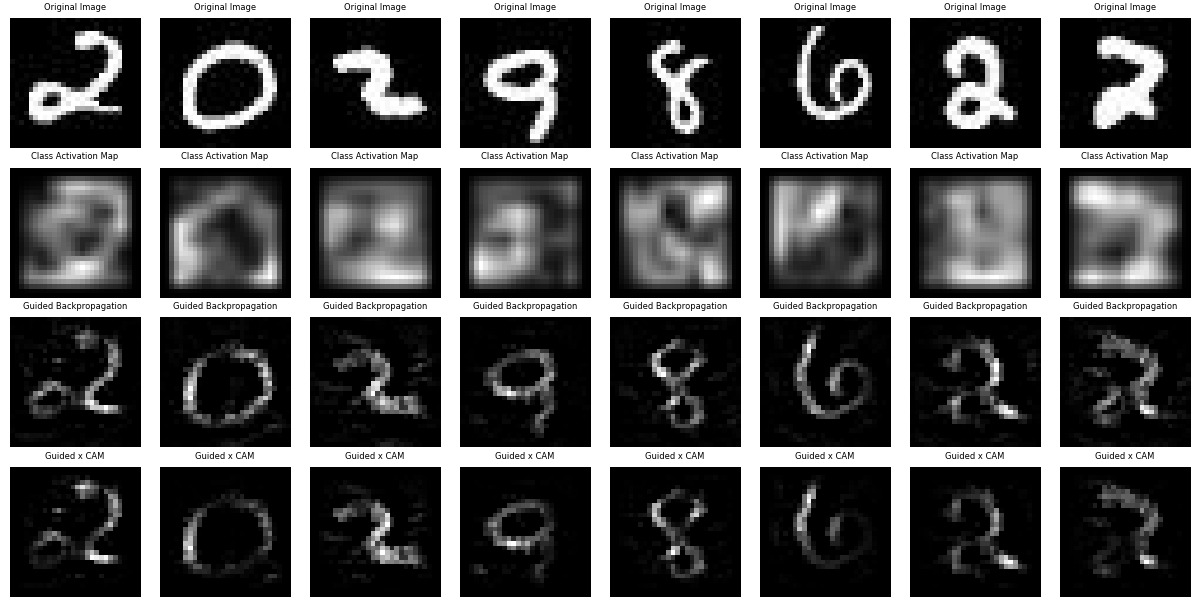
\includegraphics[width=1\linewidth]{../output.png}
\label{fig:output}
\caption{Output from T12902101\_a4.py}
\end{figure}

\subsection{Description of the parameter settings and the implementation}
\begin{itemize}
    \item parameter settings\begin{itemize}
        \item[.] model parameters: as given\begin{itemize}
            \item input shape: (N, C, H, W) = (1, 1, 28, 28)
            \item after first convolutional layer and a maxpool layer: (N, C, H, W) = (1, 10, 12, 12)
            \item after the second (also the last) convolutional layer: (N, C, H, W) = (1, 10, 8, 8), so the feature map resolution is 8x8
        \end{itemize}
        \item[.] padding size after obtaining 8x8 Grad-MAP: for each side(1, 1, 1, 1)
        \item[.] Interpolate mode after padding: Bilinear(same as the given \href{https://arxiv.org/pdf/1610.02391.pdf}{paper}\footnote{Grad-CAM: Visual Explanations from Deep Networks via Gradient-based Localization.})
        \item[.] trivial parameters when plotting are ignored
    \end{itemize}
    \item \hyperref[alg:alg]{implementation}\begin{itemize}
        \item[NOTE] Due to the absence of padding in the convolutional layers, at a resolution of 8x8, GradCAM corresponds to the central portion of the original image excluding the corners. Therefore, each side of the GradCAM would be padded by one unit before being applied to bilinear interpolation. This operation would give the final outcome a positive impact.
    \end{itemize}
\end{itemize}
\begin{algorithm}[p]
\caption{Guided Grad-CAM Generation Algorithm}
\begin{algorithmic}[1]
\State $model\gets$Initialize a model of provided neural network class, load pre-trained model weights, and set its mode to evaluate
\State $out\_channels \gets$ Output channel count of the last convolutional layer in the neural network
\State $feature\_maps$ $\gets$ Activations of the last convolutional layer as raw feature maps
\State $u, v \gets$ Height, width of the output from last convolutional layer
\State $h, w \gets$ Height, width of the testing image
\State 
\Procedure{ForthBack}{$img$}
    \State $output\gets \Call{Forward}{model,img}$ \Comment{Perform forward pass through the model}
    \State $onehot\gets \Call{GetOneHotOutput}{output}$
    \State \Call{Backward}{$output$, $onehot$} \Comment{Calculate gradients with interest}
\EndProcedure
\State
\Procedure{GenerateGradCAM}{$img$}
    \State \Call{ForthBack}{img} \Comment{Forward pass and backpropagation}
    \State $\nabla_{feature\_maps} \gets \Call{GetGradients}{feature\_maps}$
    \For{$k=0\text{ to }out\_channels-1$}
        \State $\nabla^k \gets \nabla_{feature\_maps}^k$ \Comment{Gradients for the k-th feature map}
        \State $\alpha_k \gets \frac{1}{u\cdot v}\sum\limits_{i=0}^{u-1}\sum\limits_{j=0}^{v-1}\nabla^k_{i,j}$ \Comment{Calculate weight (importance) for the k-th feature map}
    \EndFor
    \State $grad\_CAM \gets \sum\limits_{k=0}^{out\_channels-1}\Call{ReLU}{\alpha_k\cdot feature\_maps_k}$
    \State $grad\_CAM \gets \Call{Pad}{grad\_CAM,1}$
    \State $grad\_CAM \gets \Call{BilinearInterpolate}{grad\_CAM, h, w}$
    \State \Call{ZeroOutGradients}{\text{model}}
    \State \textbf{return} $grad\_CAM$
\EndProcedure
\State
\Procedure{BackpropGiude}{$grad_{input}, \dots$}
    \State $grad_{positive}\gets \Call{ReLU}{grad_{input}}$
    \State \textbf{return} $grad_{positive}$
\EndProcedure
\State
\Procedure{GuidedBackprop}{$img$}
    \State Enable gradients computation for the input image
    \State \Call{ForthBack}{$img$} \Comment{Forward pass and Execute guided backpropagation}
    \State $guided\_grad \gets \Call{GetGradients}{img}$
    \State \textbf{return} $guided\_grad$
\EndProcedure
\State
\Procedure{GenerateGuidedGradCAM}{$image$}
    \State $grad\_CAM\gets\Call{GenerateGradCAM}{image}$
    \For{$layer \in \Call{children}{model}$}
        \State $\Call{Register\_backward\_hook}{layer, BackpropGuide}$
    \EndFor
    \State $grad\_grad\gets\Call{GuidedBackprop}{image}$
    \State $guided\_CAM \gets guided\_grad \odot grad\_CAM$ \Comment{Element-wise multiplication}
    \State \textbf{return} $guided\_CAM$
\EndProcedure
\end{algorithmic}
\label{alg:alg}
\end{algorithm}

\section{Before executing \texttt{T12902101\_a4.py}}
Please note that I changed the file paths to make my assignments directory organized. Change them before you run the code. 

\begin{lstlisting}
# line 43
model.load_state_dict(torch.load("../mnist_model.pth", map_location="cpu"))
...
    raw_image = Image.open(f"../data/my_images/image_{i}.jpg")  # line 69
\end{lstlisting}

By the way, images of \texttt{"../data/my\_images/image\_i.jpg"} are created after executing \href{https://github.com/LazySheeeeep/Trustworthy_AI-Assignments/blob/main/data/transform_my_images.py}{this code}, which would transform my raw testing data \texttt{47\_data.json} into grey images and save them to that path. For convenience, I packed my testing images together at \texttt{./my\_images}.
%  \cite{selvaraju_grad-cam_2020}
% \bibliographystyle{alpha}
% \bibliography{gradcampaper}
\end{document}